\section{Grupos funcionales y jerarquías}

En esta fase, una vez definidos los elementos de datos y funcionales, vamos a
organizarlos agrupándolos en unidades funcionales que nuestras personas el
trabajo en una tarea y la transición entre tareas. Para mostrarlo de manera más
visual hemos realizado un diagrama en árbol, para el que hemos usado el
programa \underline{\href{https://www.drawio.com/}{draw.io}}. Tras un análisis, 
hemos obtenido el resultado que observamos en la figura \ref{fig:jerarquias}, el cuál explicamos a 
continuación:

\subsection{Jerarquías}

\subsubsection*{Inicial}

La primera jerarquía, la cuál podemos observar en la figura \ref{fig:jerarquias1}, es la de buscar y
reservar viajes, la funcionalidad principal de nuestra aplicación. En el apartado \textit{Inicio}
debemos elegir el origen, destino, fecha de ida, fecha de vuelta, número de
acompañantes y pinchar en el botón de buscar. Una vez pinchado el botón de buscar, nos lleva al
\textit{Comparador}, que nos muestra las diferentes opciones de viaje para la ida y la vuelta y que podemos
ordenar por precio y duración. Una vez seleccionado cómo lo queremos ordenar los muestra los viajes
según el criterio elegido. También se pueden filtrar por duración, escalas y accesibilidad. Al
igual que en la ordenación nos mostraría las opciones resultantes tras el filtrado. Durante todo
este proceso tenemos la opción de visualizar la información del viaje de cada uno de
los trayectos mostrados. Una vez seleccionados los viajes deseados, debemos elegir los asientos,
rellenar los datos de los pasajeros, seleccionar los servicios adicionales y confirmar los datos.
Una vez se haya realizado el paso anterior, se procederá al pago. En el apartado \textit{Pago} se
deberán rellenar los datos de pago (tarjeta o \textit{PayPal}) y confirmarlo. Una vez completado el pago,
la reserva ya está confirmada.

\begin{figure}
      \centering
      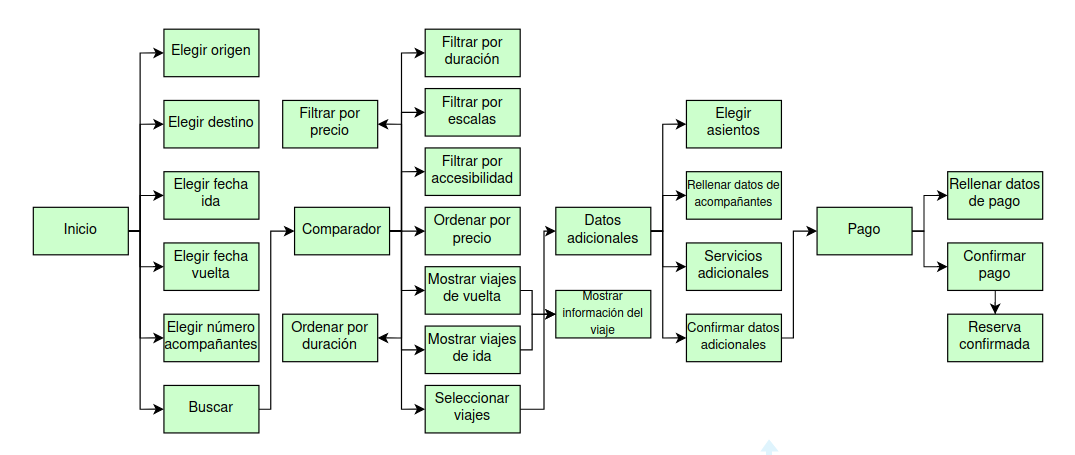
\includegraphics[width=0.8\linewidth]{./Imagenes/jerarquia-viaje.png}
      \caption{Diagrama de jerarquía para la reserva de un viaje}
      \label{fig:jerarquias1}
\end{figure}

\subsubsection*{Perfil}

En el apartado \textit{Perfil}, cuya jerarquía podemos ver en la figura \ref{fig:jerarquias2},
podemos acceder pulsando el botón de la esquina superior derecha en caso de haber iniciado sesión. Cuenta
con las siguientes opciones:

\begin{itemize}
      \item \textit{Modificar datos.} Nos muestra los datos actuales con la opción de cambiarlos. Después
            de modificarlos debemos confirmar los cambios.
      \item \textit{Mostrar los datos del usuario.} Nos muestra los datos personales del usuario como
            el nombre, los apellidos, el correo electrónico, el teléfono, la fecha de nacimiento
            y el DNI.
      \item \textit{Cerrar sesión.} Cierra la sesión del usuario actual.
      \item \textit{Mis reservas.} Muestra la información de las reservas pasadas y de las activas. Así
            como, la posibilidad de modificar y cancelar las reservas activas. Si se desea
            modificar la reserva, te da la posibilidad de elección de asientos, cambiar los datos
            de los pasajeros y seleccionar servicios adicionales. Después de modificar los datos
            deseados, debemos confirmar los cambios. Si se desea cancelar la reserva, se debe
            indicar cual/es de los billetes se quiere anular, el motivo y confirmar la cancelación.
\end{itemize}

\begin{figure}
      \centering
      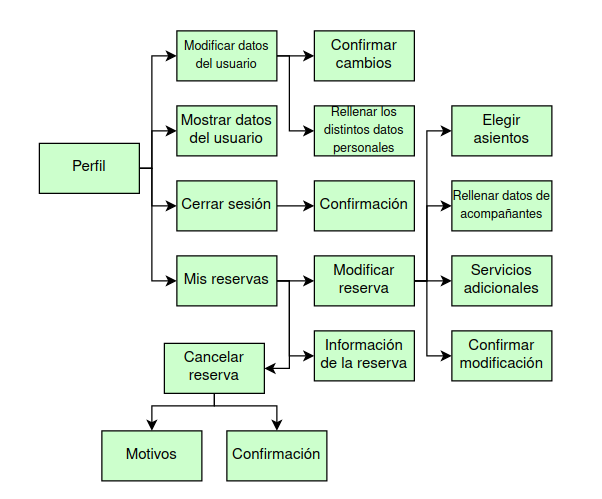
\includegraphics[width=0.8\linewidth]{./Imagenes/jerarquia-perfil.png}
      \caption{Diagrama de jerarquía para \textit{Perfil}}
      \label{fig:jerarquias2}
\end{figure}

\subsubsection*{Iniciar sesión}

En caso de querer iniciar sesión habría que pulsar el botón de la esquina superior derecha no teniendo
sesión iniciada. De esta manera accederíamos a la jerarquía de la figura \ref{fig:jerarquias3}, que
cuenta con las siguientes características.

\begin{itemize}
      \item Si el usuario tiene una cuenta, le pedirá el correo electrónico y contraseña antes
            de confirmar el inicio que le llevará a la página web con la sesión iniciada.
      \item Si el usuario no tiene cuenta, le dará la opción de crearla. Le llevará a la página
            de registro donde tendrá que rellenar los datos personales pedidos y confirmar el
            registro. Una vez creada la cuenta, iniciará sesión con sus credenciales.
\end{itemize}

\begin{figure}
      \centering
      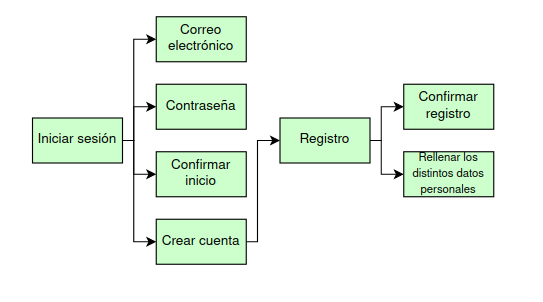
\includegraphics[width=0.8\linewidth]{./Imagenes/jerarquia-registro.png}
      \caption{Diagrama de jerarquía para el inicio de sesión y el registro}
      \label{fig:jerarquias3}
\end{figure}

\subsubsection*{Soporte/FAQ}

Desde cualquier punto de la aplicación se podrá acceder tanto a la pantalla \textit{Soporte} como
a la de \textit{Preguntas frecuentas}. La jerarquía de éstas se pueden ver en la figura \ref{fig:jerarquias4}.
Contamos con un apartado de \textit{Preguntas frecuentes} en el que podemos encontrar las preguntas
más frecuentes realizadas por los usuarios. En el caso de que la duda o cuestión del usuario no se
encuentre resuelta en el apartado anterior, también se cuenta con el apartado \textit{Soporte}. En
este apartado podemos encontrar tres opciones dependiendo de las necesidades del usuario:

\begin{itemize}
      \item \textit{Teléfono.} Nos muestra el número de contacto, así como, el horario de
            atención.
      \item \textit{Chat.} Nos permite enviar y recibir mensajes a atención al usuario.
      \item \textit{Mensajería.} Nos pide los datos de contacto como el nombre, el correo
            electrónico, el número de reserva y el mensaje que queremos envíar, para posteriormente
            enviarlo al equipo de atención al cliente.
\end{itemize}

\begin{figure}
      \centering
      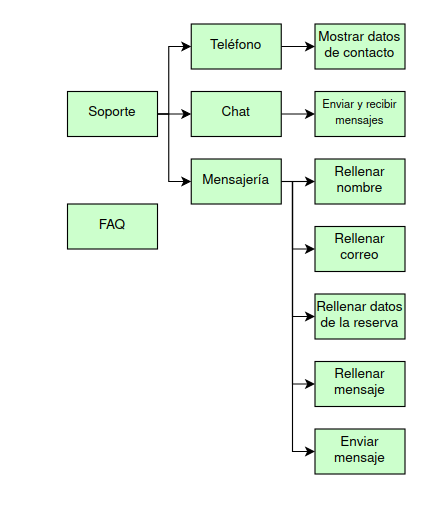
\includegraphics[width=0.8\linewidth]{./Imagenes/jerarquia-soporte.png}
      \caption{Diagrama de jerarquía para \textit{Soporte} y \textit{Preguntas frecuentes}}
      \label{fig:jerarquias4}
\end{figure}

\subsection{Principios y patrones usados}

Algunos de los principios que hemos usado a la hora de diseñar son los siguientes:

\begin{itemize}

      \item \textbf{Principio de proximidad.} Este principio nos dice que cuando ciertos elementos están próximos, el cerebro interpreta
            que están relacionados. Esto facilita tanto el aprendizaje como la memoribiliadad de cara al usuario. Este principio lo usamos en prácticamente
            todas las ventanas, ya que la mayoría poseen varios botones u opciones relacionadas que son agrupables.
      \item \textbf{Consistencia interna.} Dentro de la aplicación mantenemos todos los elementos que posean la misma funcionalidad con apariencias iguales
            o similares. Esto lo hemos aplicado en el los fondos de la aplicación, en el uso de las \textit{Cards} para los viajes, en la fuente de letra, los
            botones, etc. De esta manera, se facilita que el usuario perciba las potencialidades de los elementos de la interfaz.
      \item \textbf{Consistencia externa.} Es importante mantener funcionalidades que se encuentra en otros sistemas para que los usuarios usen sus conocimientos
            de esos sistemas y no haya fricción cognitiva. Esto lo vemos por ejemplo en el \textit{Perfil}, que como en la mayoría de aplicaciones se encuentra en la parte
            superior a la derecha.
      \item \textbf{Ley de Hick.} Esta ley nos dice que el tiempo que hay que invertir para tomar una decisión incrementa con el número de opciones disponibles y la complejidad
            de éstas. Por eso, es importante dividir las tareas complejas en varios pasos. Esto lo aplicamos al realizar la reserva de un viaje, ya que ésta cuenta de varios
            pasos (\textit{Comparador}, donde se muestran todos los viajes disponibles; \textit{Reserva}, donde el usuario pone los datos adicionales del viaje, como los asientos
            o el resto de servicios; \textit{Pago}, donde el usuario rellena los datos referentes al pago para confirmar la reserva).
      \item \textbf{Principio de libertad y control del usuario.} En todos los aspectos intentamos dar el máximo control y libertad al usuario. Esto lo hacemos poniendo un botón para volver a la anterior
            pantalla en la mayoría de páginas y, por ejemplo, permitiendo la modificación o cancelación de las reservas hechas.
      \item \textbf{Principio de cierre.} Este principio nos dice que nuestro cerebro tiene tendencia a identificar patrones secuenciales, que constan de planteamiento, desarrollo y cierre,
            el cuál debe ser natural, una continuación del proceso que estábamos siguiendo. Este principio lo usamos por ejemplo en las pantallas en las que hay que hacer \textit{scroll} hacia abajo,
            dejando algún elemento entrecortado para mostrar al usuario que hay más elementos debajo.
      \item \textbf{Regla del \textit{peak-end}} Esta regla es un sesgo cognitivo que nos dice que los momentos intensos y los momentos finales de
            de una experiencia tienen gran importancia al recordar eventos pasados, por eso es importante cuidar estos momentos. Al finalizar un proceso laborioso como
            puede ser el de reserva de un viaje, mostramos una pantalla de que ha sido correctamente reservado, dando una sensación de tranquilidad al usuario
            al final del proceso.

\end{itemize}

Dentro de cada una de las ventanas explicaremos en más profundidad los principios usados para cada ventana en concreto.